\section{Introduction}

%Following End-to-End paper style
%Target: 1.5 page

%========

%Part 1: What is KBQA
%KB intro
%KBQA Target

%1. KB introduction
%In recent years, lots of large-scale structured knowledge bases (KB)
%are manually curated by community efforts.
%%knowledge bases are large-scale structured databases.
%Knowledge bases are typically represented in the form of a graph,
%where unique named entities, concepts and types are connected
%using predefined predicates as edges.
%%Thus powerful resource for organizing open domain facts 
%%2. KBQA task
The knowledge-based question answering (KBQA) is a task which 
takes a natural language question as input and returns a factual answer 
using structured knowledge bases
%organizing open domain facts in the real world,
such as Freebase~\cite{bollacker2008freebase},
YAGO~\cite{suchanek2007yago} and DBpedia~\cite{auer2007dbpedia}.
%organize massive open domain facts in the real world,
%and make KBQA an open and popular research task,
%attracting interests from both NLP and IR communities.
%Goal of KBQA: taking NL language as input, return answers or query structures
%and then leveraging query language like SPARQL.
%KBQA: more and more attention
%3. Interesting and open research task
%The benchmark datasets such as
%Free917~\cite{cai2013large}, WebQuestions~\cite{berant2013semantic},
%ComplexQuestions~\cite{bao2016constraint} and SimpleQuestions~\cite{bordes2015large}
%are widely used in most of the recent KBQA work.
%========
%Part 2: Examples, talk about our focus: NN-based approach to answer the question.
%what's the second longest river in USA?
% We can introduce it without mentioning concepts like EL, RM..
% it's the problem that we are facing.
%The questions in KBQA task are factual questions,
%since the answer of each question is an object entity\footnote{Could be type or literal value}
%of an existing subject entity in the question.
One simple example is a question like this: ``What's the capital of the United States?''
%we need to first recognize the subject named entity in the question,
%for example, \textit{united\_states} in Freebase,
%then understand the relation ``capital of'' connecting the subject and object answer,
%is represented by the predicate \textit{location.location.capital} in FB, for example.
A common answer to such question is to identify the focus entity
and the main relation predicate (or a sequence) in the question, and 
map the question to a triple fact query ($US$, $capital$, $?$) over KB.
The object answers are returned by executing the query.
The mapping above is typically learned from question-answer pairs
through distant supervision.
%Simple: denoted by a single fact
%Generally speaking, To solve the KBQA task, 
%find the fact ($subj$, $pred$, $obj$) where subject is the entity
%and the pred is the predicate that the question describes.
%To answer the question,
%goal is to find the related predicates

\begin{figure}[th]
	\centering
	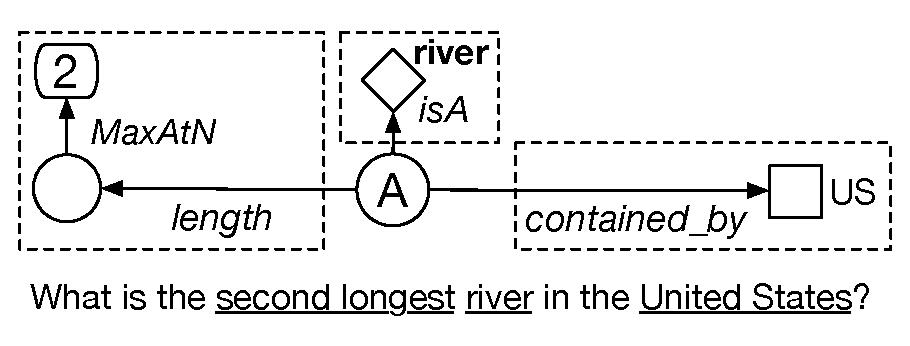
\epsfig{file=figures/intro.eps, angle=0, width=1.0\columnwidth}
	%\scalebox{0.3}{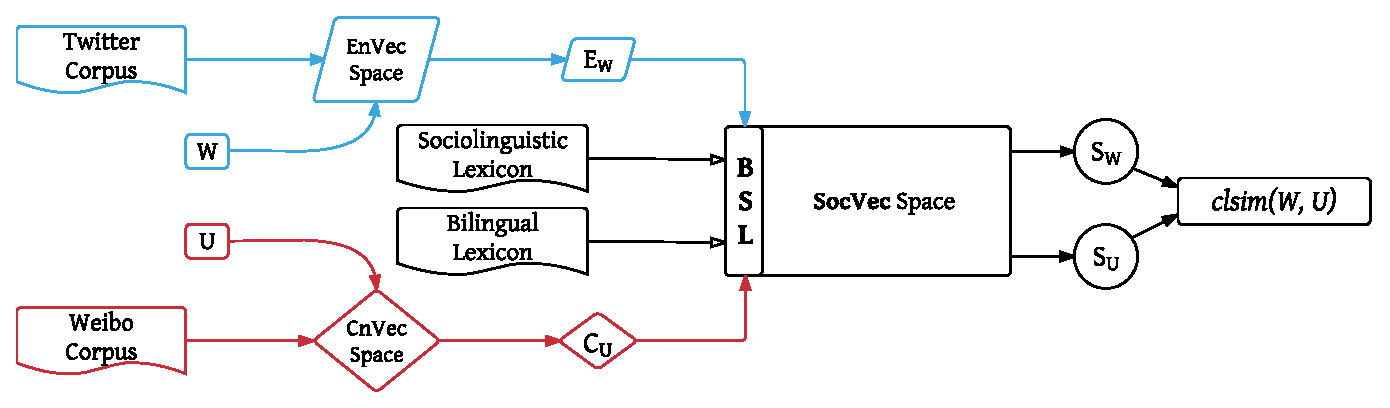
\includegraphics{overview.eps}}
	\caption{Running example of complex question.}
	\label{fig:intro}
\end{figure}

While the above question can be answered by querying
a single predicate or predicate sequence in
the KB, many other more complex questions cannot, e.g. the question
in \figref{fig:intro}.
%However, KBQA is not a trivial task,
%because we are facing questions more complex than the previous case,
%\XS{Why we are facing complex now? This ``However'' is a little bit sudden}
%where the semantics of the question is not expressed by a single triple fact.
%One question could have several focus entities,
%like ``Who played Bilbo Baggins in the Hobbits'',
%where both the character and the film are focus entities.
%Our running example in \figref{fig:intro} is even more complex,
To answer the question ``What is the second longest river in United States'',
we need to infer several semantic clues:
1) the answer is contained by United States;
2) the answer is a river;
3) the answer ranks second by its length in descending order.
Thus, multiple predicates are required to constrain the answer set,
and we call such questions ``complex questions'' throughout this paper.

%and the ordinal information in 3) cannot even be translated into 
%an existing triple fact.
%We call them complex questions, since these questions are 
%These two questions can not be answered by a single 
%($subj$, $pred$, $obj$) fact,
%thus we call it ``complex questions''.
%According to statistics reported by Bao et al.~\shortcite{bao2016constraint},
%15\% questions in WebQuestions~\cite{berant2013semantic}, which is a 
%popular KBQA dataset, are complex.
%and the ComplexQuestions dataset is designed for measuring the quality
%of KBQA systems on the complex scenario, where all questions are complex.
%In this paper, we aim at a better performance for answering complex questions.


%Around 15\% questions in WebQuestions dataset belong to the complex category,
%and the ComplexQuestions dataset is fully built upon this kind of questions.
%%4. real example
%For example in \figref{fig:complex-example},
%the question ``What is the second longest river in China?'' is a typical complex question,
%including one focus mention ``China'', the target type mention ``river''
%as well as the ordinal indicator ``second longest''.
%%5. detail semantics
%In order to perfectly answer this question, three different semantic information should be inferred:
%1) the answer is contained by China;
%2) the answer is a river;
%3) the answer ranks 2nd by the river length attribute.
%%corresponding to different semantic components in the complex query graph.
%
%
%not trivial,
%facing complex questions
%rich semantics
%
%Challenge v.s. simple questions:
%more candidates, complex generation step, 


%%1. what's simple
%There are two main steps in the KBQA task: focus recognition and relation detection.
%The first one recognizes the focus entities of the question and link it to the KB,
%and the latter step aims at identifying the semantic relationship between the focus entities and the target answer.
%The relationship is usually represented by the predicate in the KB.
%We call a question ``simple'', if it can be answered based on a single KB predicate connecting
%one focus entity and the answer.
%%2. what's complex
%However, the KBQA is not a trivial task, because a large number of questions
%hold richer semantic information.
%Except for the single focus entity in the question,
%we can find extra focus entities, target entity types, numbers, datetimes,
%or even ordinal and aggregative indicators.
%Therefore, we call them ``complex'' questions.
%%3. percentage of complex questions
%Around 15\% questions in WebQuestions dataset belong to the complex category,
%and the ComplexQuestions dataset is fully built upon this kind of questions.
%%4. real example
%For example in \figref{fig:complex-example},
%the question ``What is the second longest river in China?'' is a typical complex question,
%including one focus mention ``China'', the target type mention ``river''
%as well as the ordinal indicator ``second longest''.
%%5. detail semantics
%In order to perfectly answer this question, three different semantic information should be inferred:
%1) the answer is contained by China;
%2) the answer is a river;
%3) the answer ranks 2nd by the river length attribute.
%%corresponding to different semantic components in the complex query graph.
%The corresponding query graph is the structural combination of these semantic components.

%========

%Part 3: KBQA Branches
%Semantic Parsing: Focus on Explicit Query Structure
%Information Retrieval


%1. Two parts
%The state-of-the-art methods for the KBQA task can be categorized into two branches.
%%2. Information Retrieval (show papers)
%The first branch is based on information retrieval (IR),
%which focus on the target answer directly.
%Candidate answers are retrieved from KB using coarse-level relation extraction,
%then the model attempts to select correct answers from the candidate set
%via binary classification or ranking techniques.
%Features of IR-based methods mainly encode whether a semantic assocation exists
%between the question surface and context information of the answer in KB,
%such as its types, predicates and neighbour entities.
%Since gold answers are always available in training data,
%IR-based methods are direct supervised and thus easier to train.
%The weakness is that, the semantic meaning of the question
%is hid in large amounts of features, which is less intuitive.
%Besides, fetures in IR methods are hard to handle compositional semantics.
%
%%3. Semantic parsing (show papers)
%The second branch is based on semantic parsing technique (SP), which focuses on
%learning a semantic parsing tree or equivalent query structure
%\footnote{We use the term ``query structure'' to represent semantic parsing tree throughout the paper.}
%that represents the semantics of the question.
%Semantic parsing trees can be translated into SPARQL queries,
%hence target answers are returned by executing the query over KB.
%Parsing trees provide clear semantic meanings of questions without ambiguity,
%and it's human-readable.
%Due to the lack of annotated semantic parsing trees of questions in training data, 
%SP-based approaches are usually distant supervised.
%
%========

%Part 4: NN into QA model & Schema Encoding

%In order to answer complex questions, it's crucial to learn the
%compositional semantic meaning of the question,
%so our research focuses on the SP with NN technique.

%lies in understanding the compositional semantic meanings

For answering complex questions, it's more important to understand the compositional
semantic meanings of the question.
%rather than directly outputting answer entities.
As a classic branch of KBQA solutions, semantic parsing (SP) technique
%Therefore, our research work is based on the semantic parsing (SP) technique
~\cite{berant2013semantic,yih2015semantic,reddy2016transforming,hu2018answering}
aims at learning semantic parse trees or equivalent query graphs
\footnote{The term ``query graph'' is interchangeable
with ``query structure'' and ``semantic parsing tree'' throughout this paper.}
for representing semantic structures of the questions.
For example in \figref{fig:intro}, the query graph forms a tree shape.
The answer node $A$, serving as the root of the tree,
is the variable vertex that represents the real answer entities.
The focus nodes (\textit{US}, \textit{river}, \textit{2nd})
are extracted from the mentions of the question,
and they constrain the answer node via predicate sequences in the knowledge base.
%and the answer node is connected to these nodes via predicate 
%sequences in the knowledge base.
%SP-based approaches first generate candidate graphs using
%bottom up parsing~\cite{berant2013semantic,cai2013large}
%or staged query generation methods~\cite{yih2015semantic,bao2016constraint}, 
%then predict the best graph by calcuating the semantic similarity of the question.
%Final answers are produced by executing the SPARQL query (shown in \figref{fig:intro})
%translated from the query graph.
Recently, neural network (NN) models have shown great promise in
improving the performance of KBQA systems,
and SP+NN techniques become the state-of-the-art on several KBQA datasets
~\cite{qu2018question,bao2016constraint}.
According to the discussion above, 
our work extends the current research in the SP+NN direction.



%1. to answer compq: understand semantic meaning rather than
%2. A main branch: SP
%   focus on build query graph.
%   refer to figure 1, tree
%3. Sp learn the best graph, and outpu answer by querying FB
%4. recently, NN based model: encode and compare style, the similarity in hidden space.
%5. SOTA (WebQ, CompQ, SimpQ)
%6. Based on the advts, lies in the SP+NN framework to answer complex questions.


%The NN-based methods avoid feature engineering in both SP- and IR- framework,
%and performance better than traditional methods.

%%4. challenge: candgen
%\KZ{Simplify these two challenges significantly.}
%We face two key challenges for answering complex questions.
%First, there is a large searching space to collect candidate query structures.
%For simple questions, the query structure is limited to 
%a single predicate connecting the focus entity and the answer.
%However, as illustrated in \figref{xxx},
%the query structure of a complex question has a tree shape with multiple edges,
%we can generate different candidates exponentially larger than
%the size we generated from simple questions.
%%4-1. other works
%Traditional semantic parsing approaches partially tackle the problem by
%introducing a ``bridge'' operation to merge simple facts into tree structure
%~\cite{berant2013semantic},
%or predefine a number of parsing templates with branches~\cite{bast2015more},
%Candidate structures can be translated from dependency parsing of the question~\cite{reddy2016},
%but it's highly relies on the parsing accuracy,
%and the translation rules need much human prior knowledge.
%There are approaches to circumvent the problem of candidate generation.
%For example, 
%Xu et al.~\shortcite{xu2016question} generated candidates in the form of single fact,
%and leverage unstructured text information to verify whethe a candidate answer
%satisfies other semantic constarints in the question.
%This approach is out of our discussion,
%as it can be regarded as a post-process step in the majority of KBQA frameworks.
%%4-2. yih & bao
%Recently, stagged query structure generation is a technique proved to be effective
%in research works~\cite{yih2015semantic,bao2016constraint}.
%The intuition is to generate query structure in step-by-step extension:
%starting from a focus entity extracted from the question, then explore candidate paths
%to the answer entity, and attach constraint paths in a depth-first search manner.
%
%Staged generation is proved to be effective and used in xxx research works.
%The difference: rules applied for particular constraints.
%
%%yih proposed a staged candidate generation scheme.
%%Based on candidate entities, search from one entity, and add constraints to the tree from other entity.
%%Bao is similar framework, considers entity / type / time / ordinal constraints with few handcrafted rules.
%%stage generation proves to be effective

%5. challenge: schema repr

%NN framework follows encoder-comp framework,
%where deep nerural networks encode both q and paths into a common embedding space,
%and calculate by cosine similarity.


The common step of SP-based approaches is to first collect candidate query graphs using
bottom up parsing~\cite{berant2013semantic,cai2013large}
or staged query generation methods~\cite{yih2015semantic,bao2016constraint}, 
then predict the best graph mainly based on the semantic similarity with the 
given question. Existing NN-based methods follow an encode-and-compare 
framework for answering simple questions,
where both the question and the predicate sequence are encoded as semantic vectors
in a common embedding space, and the semantic similarity is calculated by the cosine score
between vectors.
In order to define the similarity function between one question and a complex query graph,
an intuitive solution is to split the query graph into multiple semantic components,
as the predicate sequences separated by dashed boxes in \figref{fig:intro}.
Then previous methods can be applied for modeling the similarity between the question
and each part of the graph.
%~\cite{yih2015semantic,bao2016constraint,xu2016question}.
However, such approach faces two limitations.
First, each semantic component is not directly comparable with the whole question,
since it conveys only partial information of the question.
%TODO: maybe add more here?
%first: part of semantic of the whole sentence,
%how to encode the sentene w.r.t the components?
%attention mech or carefully designed context pattern aims to solve
%but not carefully investigated.
Second, and more importantly, the model encodes different components separately,
without learning the representation of the whole graph,
hence it's not able to capture the compositional semantics in a global 
perspective.
%The first challenge is how to encode a complex query graph into embedding space.
%Previous works handle the challenge by
%splitting a query graph into multiple predicate sequences,
%then encoding each sequence using convolution or recurrent neural networks
%This solution regards the query graph as a set of independent semantic components,
%but is not able to capture the compositional semantics in a global perspective.

%%find a representation to a complex query structure.
%%measure the similarity between q and schema.
%%5-1. other works: path only, including bao
%For answering simple questions, 
%previous works proposed methods based on convolutional or recurrent neural networks
%~\cite{lukov,yin,yu},
%since candidate query structures are in the form of predicate sequences,
%but such methods are not applicable in the complex scenario.
%An alternative approach is to model the main path of candidate structures using neural networks,
%and capture semantics of constraints by lexical features or
%leave to unstructured text verification~\cite{xu2016question,yih2015semantic},
%while the semantic information is still neglected.
%%5-2. bao, close to us. ATTACK ATTACK ATTACK!!
%The method proposed by Bao et al.~\shortcite{bao2016constraint} is most similar to us:
%the candidate query structure is split into multiple predicate sequences,
%then Siamese convolutional neural networks are used to calculate the similarity score
%between each predicate sequence and a particular ``context pattern'' (substring of the question),
%and the overall score is the weighted sum of similarity scores with other simple features.
%However, this approach still has two drawbacks.
%First, as predicate sequences are encoded separately, 
%the model cannot capture the semantic interaction between different aspects
%at the vector space level.
%Second, the encode paths and constraints separately and compare with 
%different components of the question.
%
%compare with context pattern, which is not clear
%
%not a whole representation,
%not compare with the whole sentence
%but model vector different branch constraints
%the semantic interaction between clues are lost.
%and the "context pattern" is not clear, also with ad-hoc rules.
%
%\KZ{What's the limitation or problem in existing approaches to tackle
%complex questions?}
%
%%mainly attack: not treat as whole, lose interaction in hidden semantic level
%%TODO: shall we try intra-attention????
%%and also context pattern problem.

%%========
%%Part 5: Detail point: schema encoding
%%8-10 sentences
%%1. introduce the focus: schema representation
%In this work, we pay attention to the combination SP and NN approach.
%%and focus on finding the best query graph of a given question.
%%We propose a neural network approach to compute the similarity score between a question and a candidate query structure.
%%2. semantic structure encoding: target
%The cruical step is to compute the the similarity score between q representation and SP represeantation.
%%3. previous:
%Previous work have taken efforts to the problem.
%The first method (Luc, Yu) focus on the predicate path connecting the focus and the entity, 
%where the recurrent modes like Gated Recurrent Unit (GRU) and Long Short-Term Memory (LSTM)
%show the effectiveness of modeling the representation of SP.
%This method is straightforward, but it's mainly used in simple question scenarios.
%The additional constraints can be added to the query graph, but the semantic information
%is never used in the encoding step.
%The second approach (Yih,Bao) takes all semantic components into the computation step.
%The authors didn't encode the rep. of the entire structure, as instead,
%proposed a CNN-based module to measure the semantic similarity between the question
%and various components of the query structure, including its focus entity, type, predicates.
%However, the overall model is more likely to be feature-based (with handcrafted rules),
%and when computing the similarity between q and compoenents, the subsentence of q is
%selected through hard rules, which is inflexible and may cause error propagation problem.
%%and the semantic similarities serve as some feature values of the <q, sc> pair.

%========


%1. propose
In order to attack the above limitations, we propose a neural network based 
%approach to improve relation matching performance of complex question answering.
approach to improve the performance of semantic similarity measurement
in complex question answering.
%\KZ{This is the first time u mention relation matching. Do they understand
%what it is?}
%2. basic
Given candidate query graphs generated from one question,
our model embeds the question surface and predicate sequences into a uniform 
vector space.
%3. combination
The main difference between our approach and previous methods is that
we integrate hidden vectors of various semantic components
and encode their interaction as the hidden semantics of the entire query graph.
%so that the model  encodes the semantics of whole graph structure.
%4. dependency
In addition, to cope with different semantic components of a query graph,
we leverage dependency parsing information as a complementary of 
sentential information for question encoding,
which makes the model better align each component to the question.
%5. eval
%the module is able to handle both complex questions and simple questions.
The contribution of this paper is summarized below.

%%Part 6: Ours and Challenge
%%1. semantic rep for the entire query graph.
%In order to combine the advantages of the previous methods,
%we present a neural network method for modeling the semantic vector of the entire query graph.
%%2. intuition: skeleton split
%The main intuition behind our approah is to regard the complex query graph
%as a set of simple skeletons.
%%3. what's skeleton
%Generally speaking, a skeleton is a predicate path starting from a fixed node
%(entity, type, number, datetime or ordinal value) to the target answer.
%%4. what to represent skeleton
%Each skeleton describes one semantic aspect of the question,
%and the overall representaion of a query graph is the
%dynamic combination of the skeleton vectors within the graph.
%%5. attention 1: each skeleton focus on different words in the question;
%Since different skeletons focus on different words in the question,
%we adopt a word-level attention module to learn a flexible representation
%of each skeleton.
%Besides, a skeleton-level attention module helps adjust the weight between different skeletons,
%producing the final representation of the whole graph.
%It's worth mentioning that our method learns focus recognition and relation detection jointly,
%which makes our model more robust. \KQ{need examples for clarification}

%========

%Part 7: contribution

%no need explicit contribution bullet, but say we do ... in ... manner...
% kernel: embedding strategy
% than: q-rep, path-rep
% others: candgen, enrich ...



% candgen: less rules???? must be kidding me.
% model in general: interactive composing semantic components.
% model in detail: path embedding, rather than predicate word embedding?? (make use of ids and names)
% footnote: http://anonymous.for.double.blind.review

%TODO: first try compositional
%TODO: dependency as local information
%TODO: best result in CompQ by 1.9\%, competitive in WebQ and SimpQ.

\begin{itemize}
\item We propose a light-weighted and effective neural network model to solve complex KBQA task.
      To the best of our knowledge, this is the first attempt to
      explicitly encode the complete semantics of a complex 
 	  query graph (\secref{sec:rm});
\item We leverage dependency parsing to enrich question representation 
	  in the NN model, and conduct thorough investigations to 
	  verify its effectiveness (\secref{sec:qw-repr});
\item We propose an ensemble method to enrich entity linking from
      a state-of-the-art linking tool, which further improves the 
      performance of the overall task (\secref{sec:ensemble});

\item We perform comprehensive experiments on multiple QA datasets,
      and our proposed method consistently outperforms previous approaches 
	  on complex questions, and produces competitive results on 
	  datasets made up of simple questions (\secref{sec:exp}).
\end{itemize}

%1. compact v.s. separated features (composition is better than isolated calculation) (interaction) (YES INTERATCTION, HOW to state?)
%   a. traditional: yih, xu, jain: ignore or postprocess
%   b. bao: simply weighted sum
%2. "context pattern" or other clues needed to send to the other side of BiCNN (ad-hoc to determine context pattern, not clearly mentioned)
%3. no need pre-train CNN (don't think pre-train is a good choice)

%Main part in the intro:
%  how to tackle the question with multiple constraints.
%  Imitate intro from Yih, Bao, Xu, Jain, Yin(f)...
%
%Interact:
%  semantic interact: (max pooling) simple but effective
%  entity linking: interactive feature (however, not used right now)
%  
%
%RM helped by EL: raw score as evidence
%EL helped by RM: rare (RM is more reliable)
